\documentclass[
	usepdftitle=false,
	xcolor={table, dvipsnames},
	hyperref={
		pdftitle={Machine Learning per Software Engineering},
    	pdfauthor={Alessando Chillotti}
    }
]{beamer}

\mode<presentation> {

% The Beamer class comes with a number of default slide themes
% which change the colors and layouts of slides. Below this is a list
% of all the themes, uncomment each in turn to see what they look like.

%\usetheme{default}
%\usetheme{AnnArbor}
%\usetheme{Antibes}
%\usetheme{Bergen}
%\usetheme{Berkeley}
%\usetheme{Berlin}
%\usetheme{Boadilla}
%\usetheme{CambridgeUS}
%\usetheme{Copenhagen}
%\usetheme{Darmstadt}
%\usetheme{Dresden}
%\usetheme{Frankfurt}
%\usetheme{Goettingen}
%\usetheme{Hannover}
%\usetheme{Ilmenau}
%\usetheme{JuanLesPins}
%\usetheme{Luebeck}
%\usetheme{Madrid}
%\usetheme{Malmoe}
%\usetheme{Marburg}
%\usetheme{Montpellier}
%\usetheme{PaloAlto}
\usetheme{Pittsburgh}
%\usetheme{Rochester}
%\usetheme{Singapore}
%\usetheme{Szeged}
%\usetheme{Warsaw}

% As well as themes, the Beamer class has a number of color themes
% for any slide theme. Uncomment each of these in turn to see how it
% changes the colors of your current slide theme.

%\usecolortheme{albatross}
%\usecolortheme{beaver}
%\usecolortheme{beetle}
%\usecolortheme{crane}
%\usecolortheme{dolphin}
%\usecolortheme{dove}
%\usecolortheme{fly}
%\usecolortheme{lily}
%\usecolortheme{orchid}
%\usecolortheme{rose}
%\usecolortheme{seagull}
%\usecolortheme{seahorse}
%\usecolortheme{whale}
%\usecolortheme{wolverine}

%\setbeamertemplate{footline} % To remove the footer line in all slides uncomment this line
%\setbeamertemplate{footline}[page number] % To replace the footer line in all slides with a simple slide count uncomment this line

%\setbeamertemplate{navigation symbols}{} % To remove the navigation symbols from the bottom of all slides uncomment this line
}

\usepackage[utf8]{inputenc}
\usepackage[italian]{babel}
\usepackage[T1]{fontenc}
\usepackage{graphicx}
\usepackage{booktabs}
\usepackage{subcaption}
\usepackage{accents}
\usepackage{adjustbox}

\setlength{\arrayrulewidth}{0.1em}
\renewcommand{\arraystretch}{1.2}

\title[Progetto ISW2]{Machine Learning per Software Engineering} 

\author{Alessandro Chillotti}

\institute[]{Università degli studi di Roma Tor Vergata}
\date{19 Giugno 2022}

\usefonttheme[onlymath]{serif}
\graphicspath{ {./figs/} }
\definecolor{code_purple}{rgb}{0.5,0,0.35}

\begin{document}
\beamertemplatenavigationsymbolsempty
\addtobeamertemplate{navigation symbols}{}{%
    \usebeamerfont{footline}%
    \usebeamercolor[fg]{footline}%
    \hspace{1em}%
    \insertframenumber/\inserttotalframenumber
}
\setbeamercolor{footline}{fg=blue}
\setbeamerfont{footline}{series=\bfseries}

\begin{frame}
\titlepage
\end{frame}

\begin{frame}
\frametitle{Indice}
\tableofcontents
\end{frame}

\section{Introduzione}
\begin{frame}
\frametitle{Introduzione (1/4)}
\begin{block}{Contesto del progetto e terminologia (1/2)}

Nell'ingegneria del software esiste un tema importante che riguarda le previsioni di bug, ovvero il processo che ha l'obiettivo di identificare se artefatti software sono difettosi. 

Si necessita di alcune nozioni preliminari:
\begin{itemize}
\item \textit{Revisione}: ogni commit produce una revisione
\item \textit{Versione}/\textit{Release}: è una revisione che viene resa pubblica ed utilizzabile
\item \textit{Ticket}: è un evento che deve essere esaminato o un elemento di lavoro che deve essere affrontato. Contiene delle informazioni importanti:

\begin{itemize}
\item[--] \textit{Tipo}: rappresenta il tipo di lavoro che deve essere affrontato (e.g. Bug)
\end{itemize}
\end{itemize}
\end{block}
\end{frame}

\begin{frame}
\frametitle{Introduzione (2/4)}
\begin{block}{Contesto del progetto e terminologia (2/2)}
\begin{itemize}
\item \textit{Injected Version} (IV): è la versione nella quale il bug è stato inserito
\item \textit{Opening Version} (OV): è la versione nella quale si è aperto il ticket relativo al bug
\item \textit{Affected Versions} (AV): sono le versioni che sono state affette dal bug
\item \textit{Fixed Version} (FV): è la versione nella quale il bug è stato risolto
\end{itemize}
\end{block}
\end{frame}

\begin{frame}
\frametitle{Introduzione (3/4)}
\begin{block}{Problema}
Come enunciato in precedenza, nell'ingegneria del software la previsione dei bug gioca un ruolo fondamentale. In particolare, nel caso di un progetto software Java:
\begin{itemize}
\item Una classe difettosa è una classe che presenta un bug al suo interno
\item Per correggere un bug si ha bisogno di una fase di test che può essere costosa
\end{itemize}
Prevedere che una classe possa essere difettosa può permettere al tester di concentrarsi su mirate classi, senza dover spendere altri costi su classi che non sono difettose
\end{block}
\end{frame}

\begin{frame}
\frametitle{Introduzione (4/4)}
\begin{block}{Obiettivi dello studio eseguito}
Il progetto svolto è uno studio empirico finalizzato a misurare l’effetto di tecniche di sampling, classificazioni sensibili al costo e feature selection sull’accuratezza di modelli predittivi di machine learning. 

I progetti open-source utilizzati sono sviluppati dalla Apache Software Foundation:
\begin{itemize}
\item \textit{Apache Bookkeeper}
\item \textit{Apache Zookeeper}
\end{itemize}
Lo scopo della presentazione è quello di presentare i risultati:
\begin{itemize}
\item In una prima fase verranno mostrati i risultati ottenuti al variare delle combinazioni di tecniche applicate
\item In una seconda fase verrà mostrato il comportamento dei classificatori in scenari specifici
\end{itemize}
\end{block}
\end{frame}

\section{Progettazione}
\begin{frame}
\frametitle{Progettazione (1/3)}
\begin{block}{Costruzione dei dataset}
Per la costruzione dei dataset sono stati eseguiti i seguenti passi:
\begin{enumerate}
\item Combinazione dell'utilizzo delle REST api di \textit{Jira} e il tool \textit{JGit} per la costruzione della lista di versioni necessarie
\item Retrieve dei ticket di tipo bug e per ognuno di essi si tiene traccia dei file toccati. In particolare, nel caso in cui il ticket non avesse le AV, si è utilizzato il metodo proportion per stimare l'IV da utilizzare per definire le AV
\item Computazione della buggyness di ogni classe per ogni versione andando ad analizzare i dati ottenuti al passo 2
\end{enumerate}
\end{block}

\begin{block}{Caratteristiche dei dataset ottenuti}
I dataset ottenuti hanno come classe minoritaria la classe buggy:
\begin{itemize}
\item In Bookkeeper circa il 23\% di classi è buggy
\item In Zookkeeper circa l'11\% di classi è buggy
\end{itemize}
\end{block}
\end{frame}

\begin{frame}
\frametitle{Progettazione (2/3)}
\begin{block}{Metriche selezionate}
Le metriche selezionate per la realizzazione del dataset sono:
\fboxsep=0pt
\noindent{%
\begin{minipage}[t]{0.49\linewidth}
\begin{itemize}
\item \textit{Size}: numero di LOC
\item \textit{NAuth}: numero di autori di una classe
\item \textit{Max LOC added}: massimo numero di LOC aggiunte in una release
\item \textit{Churn}: differenza fra numero di LOC aggiunte e rimosse
\item \textit{AVG churn}: media della differenza fra numero di LOC aggiunte e rimosse
\end{itemize}
\end{minipage}}%
\hfill%
{%
\begin{minipage}[t]{0.49\linewidth}
\begin{itemize}
\item \textit{NR}: numero di revisioni
\item \textit{LOC added}: numero di LOC aggiunte in una release
\item \textit{AVG LOC added}: numero medio di LOC aggiunte in una release
\item \textit{Max churn}: massima differenza fra numero di LOC aggiunte e rimosse
\item \textit{Age}: età in settimane di una classe
\end{itemize}
\end{minipage}
}
\end{block}
\end{frame}

\begin{frame}
\frametitle{Progettazione (3/3)}
\begin{block}{Tecnica di classificazione}
La tecnica di classificazione utilizzata è \textit{walk forward}, quindi l'idea è che ad ogni run $i$, considerando le versioni ordinate cronologicamente, si ha che:
\begin{itemize}
\item il \textit{training set} contiene le prime $i$ - $1$ versioni
\item il \textit{testing set} contiene esclusivamente la versione $i$-esima
\end{itemize}

I classificatori utilizzati sono \textit{Random Forest}, \textit{Naive Bayes} e \textit{Ibk}. Per la loro esecuzione è stato utilizzato il tool \textit{Weka}, in particolare le API messe a disposizione da esso.
\end{block}

\begin{block}{Metriche analizzate}
Le metriche di performance di cui sono stati analizzati i valori sono la \textit{recall}, la \textit{precision}, la \textit{kappa} e l'\textit{AUC}(\textit{Area Under The Curve}).
\end{block}
\end{frame}

\section{Variabili}
\begin{frame}
\frametitle{Variabili}
\begin{block}{Variabili considerate}
Le variabili validate empiricamente sono le seguenti:
\begin{itemize}
\item come feature selection, si considera \textit{best first}
\item come balancing, si considerano :
\begin{itemize}
\item \textit{oversampling}: si aumentano le istanze della classe minoritaria fino a pareggiare il numero di istanze della classe maggioritaria
\item \textit{undersampling}: si diminuiscono le istanze della classe maggioritaria fino a pareggiare il numero di istanze della classe minoritaria
\item \textit{SMOTE}: si creano "sinteticamente" nuove istanze per la classe minoriataria
\end{itemize}
\item come cost sensitive, si considerano \textit{sensitive threshold} e \textit{sensitive learning} e la matrice dei costi prevede un costo dieci volte maggiore per un falso negativo rispetto al costo per un falso positivo
\end{itemize}
\end{block}
\end{frame}

\section{Classificatore Ibk al variare delle tecniche applicate}
\begin{frame}
\frametitle{Ibk - Risultati ottenuti (1/3)}
\begin{block}{Bookkeeper - Comportamento al variare delle tecniche}
\begin{figure}[ht!]
\frame{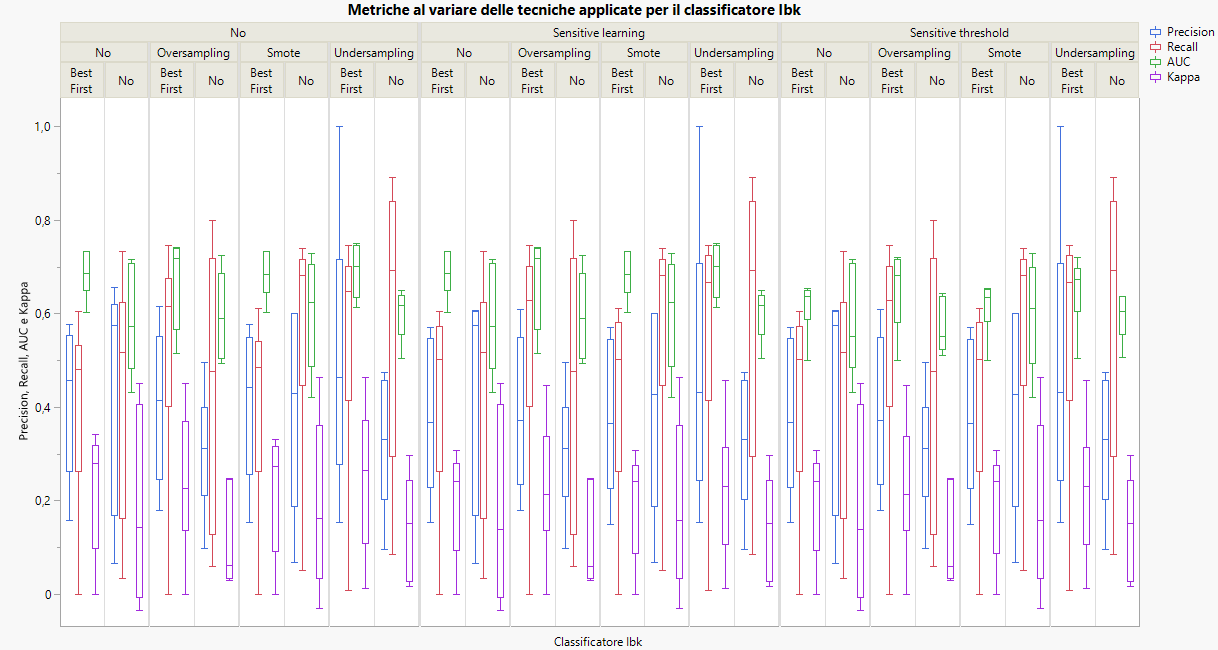
\includegraphics[width=\textwidth]{figs/bookkeeper-ibk}}
\end{figure}
\end{block}
\end{frame}

\begin{frame}
\frametitle{Ibk - Risultati ottenuti (2/3)}
\begin{block}{Zookeeper - Comportamento al variare delle tecniche}
\begin{figure}[ht!]
\frame{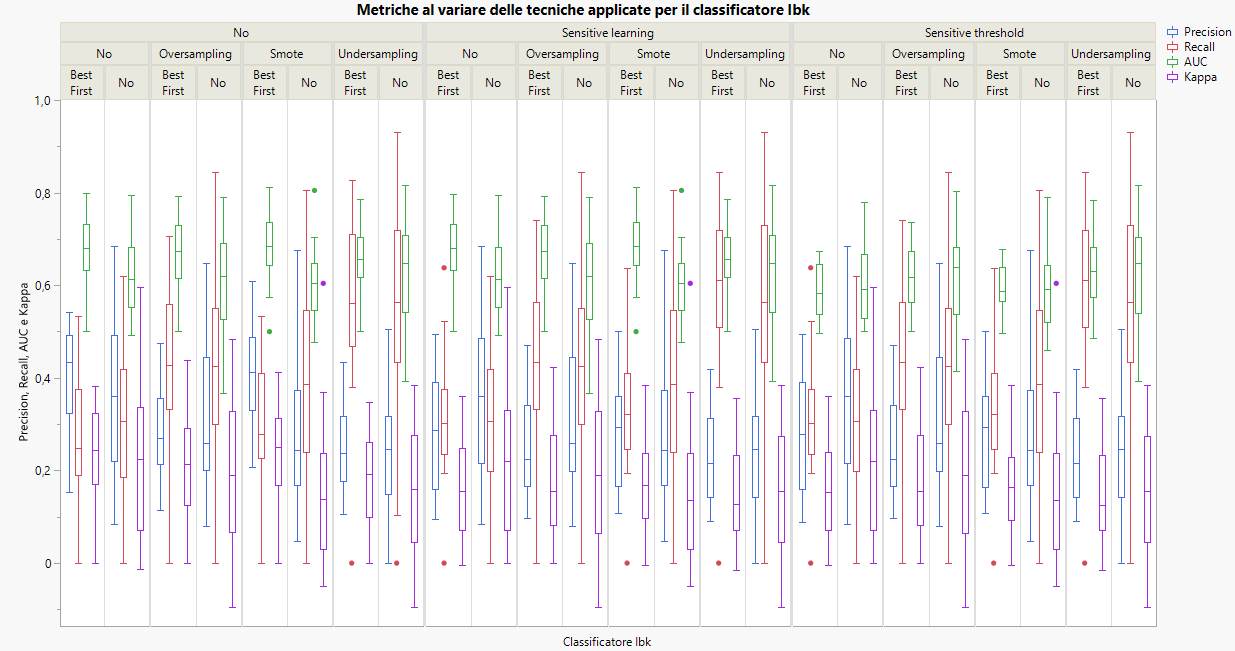
\includegraphics[width=\textwidth]{figs/zookeeper-ibk}}
\end{figure}
\end{block}
\end{frame}

\begin{frame}
\frametitle{Ibk - Risultati ottenuti (3/3)}
\begin{block}{Considerazioni riguardo il classificatore Ibk}
\begin{itemize}
\item La \textit{recall} migliora con l'applicazione di tecniche di balancing
\item La \textit{precision} peggiora quando vengono applicate tecniche di balancing e risente anche dell'applicazione di tecniche di cost sensitive
\item I risultati descritti nei primi due bullet sono attesi, in quanto un buon balancing aumenta significativamente la \textit{recall} inficiando poco sulla \textit{precision}
\item L'\textit{AUC} migliora con l'applicazione di feature selection, ma nel caso in cui si applica \textit{sensitive threshold}, in Zookkeeper, questo comportamento tende a cambiare
\item \textit{Kappa} peggiora con l'applicazione di feature selection, ad eccezioni di alcuni casi in Zookkeeper ed inoltre peggiora con l'applicazione di tecniche cost sensitive
\end{itemize}
\end{block}
\end{frame}

\section{Classificatore Random Forest al variare delle tecniche applicate}
\begin{frame}
\frametitle{Random Forest - Risultati ottenuti (1/3)}
\begin{block}{Bookkeeper - Comportamento al variare delle tecniche}
\begin{figure}[ht!]
\frame{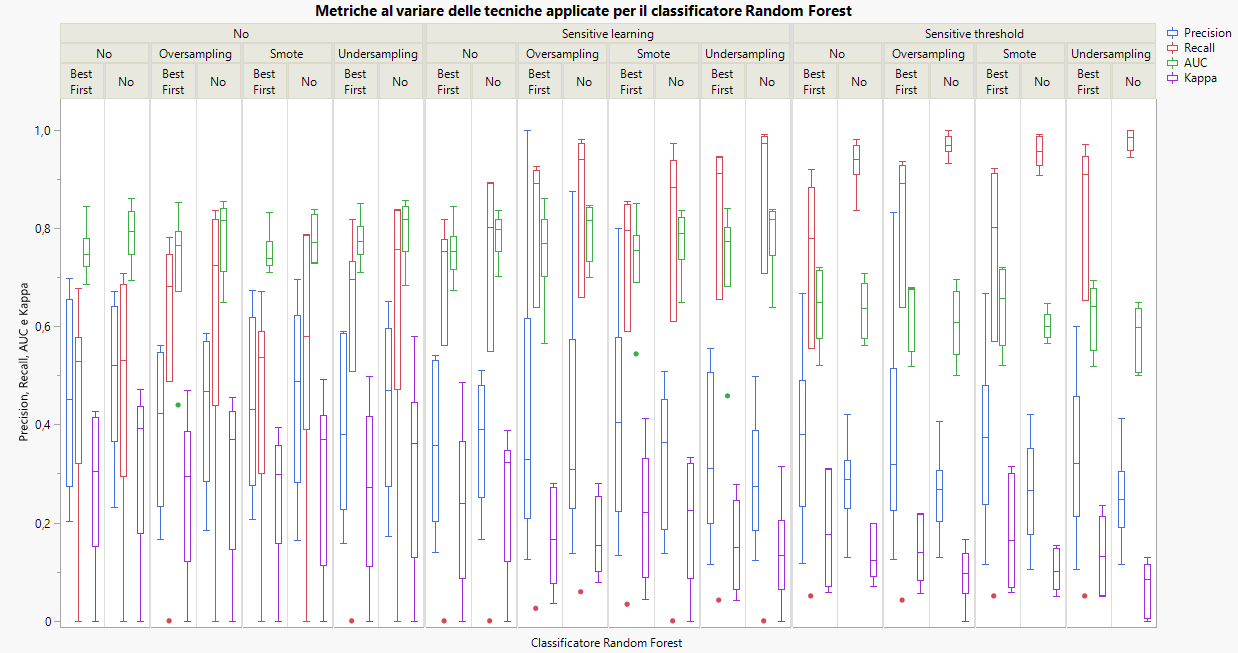
\includegraphics[width=\textwidth]{figs/bookkeeper-forest}}
\end{figure}
\end{block}
\end{frame}

\begin{frame}
\frametitle{Random Forest - Risultati ottenuti (2/3)}
\begin{block}{Zookeeper - Comportamento al variare delle tecniche}
\begin{figure}[ht!]
\frame{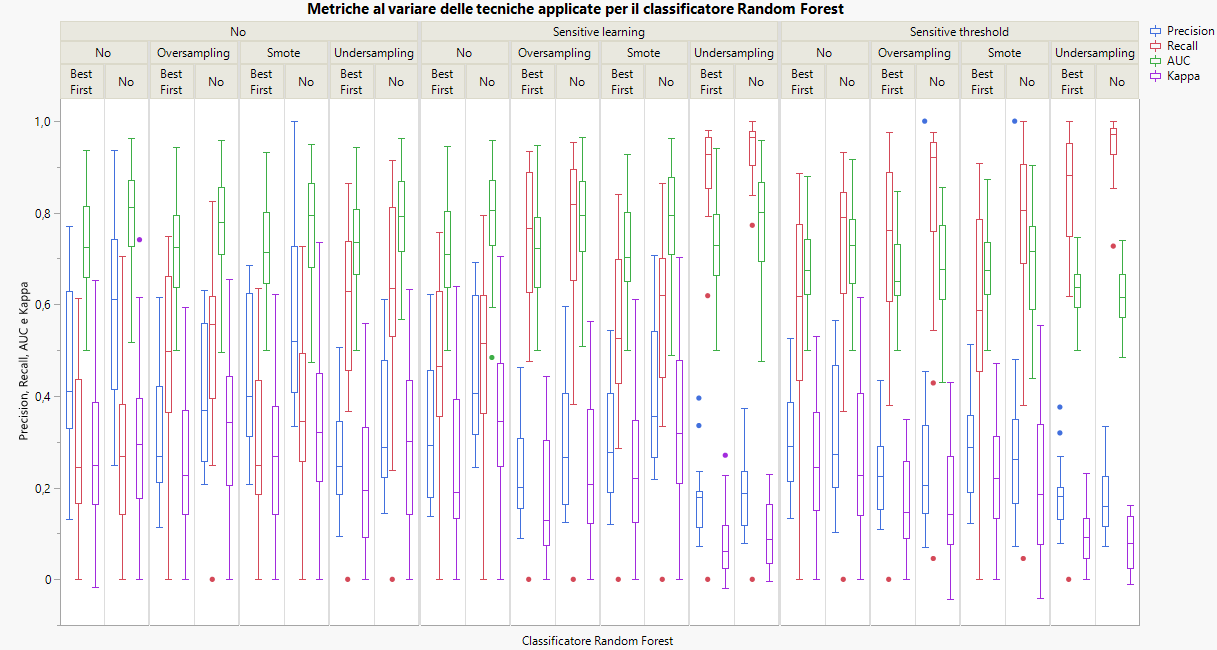
\includegraphics[width=\textwidth]{figs/zookeeper-forest}}
\end{figure}
\end{block}
\end{frame}

\begin{frame}
\frametitle{Random Forest - Risultati ottenuti (3/3)}
\begin{block}{Considerazioni riguardo il classificatore Random Forest}
\begin{itemize}
\item La \textit{recall} migliora nel caso in cui si applicano tecniche di balancing e tecniche di cost sensitive, in particolare si raggiungono valori alti nel caso di applicazione di \textit{undersampling}
\item D'altra parte, questo inficia sulla \textit{precision} ed infatti il valore di precision più alto si ha quando non vengono applicate tecniche di balancing
\item L'\textit{AUC} non viene alterata significativamente nel caso in cui viene applicato \textit{sensitive learning} rispetto al caso in cui non si applicano tecniche di cost sensitive, ma l'applicazione di \textit{sensitive threshold} porta ad un suo peggioramento
\item \textit{Kappa} non migliora con l'applicazione di feature selection, anche se nel caso in cui si applica \textit{sensitive threshold} questo comportamento tende ad invertirsi
\end{itemize}
\end{block}
\end{frame}

\section{Classificatore Naive Bayes al variare delle tecniche applicate}
\begin{frame}
\frametitle{Naive Bayes - Risultati ottenuti (1/3)}
\begin{block}{Bookkeeper - Comportamento al variare delle tecniche}
\begin{figure}[ht!]
\frame{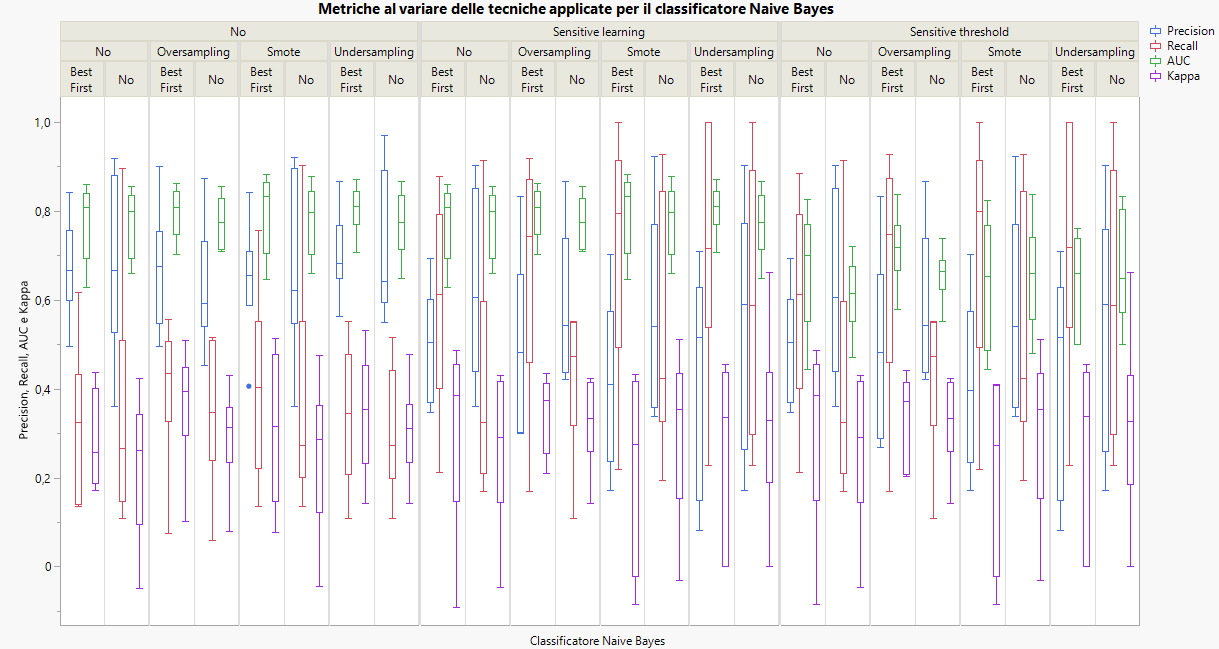
\includegraphics[width=\textwidth]{figs/bookkeeper-bayes}}
\end{figure}
\end{block}
\end{frame}

\begin{frame}
\frametitle{Naive Bayes - Risultati ottenuti (2/3)}
\begin{block}{Zookeeper - Comportamento al variare delle tecniche}
\begin{figure}[ht!]
\frame{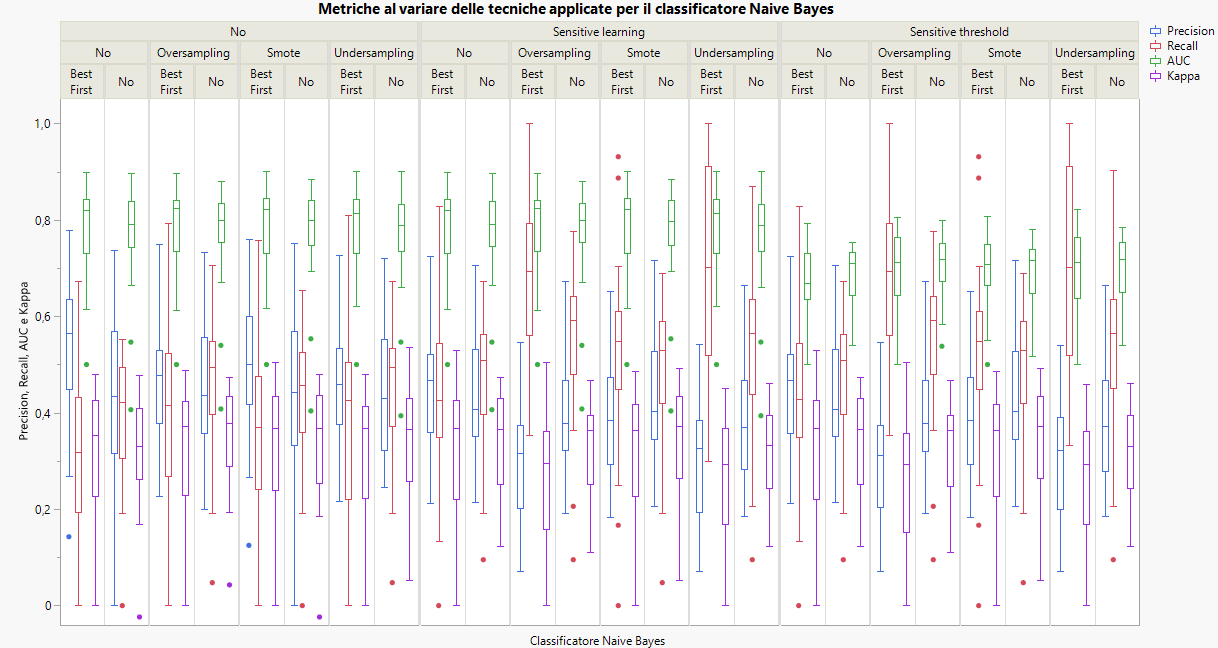
\includegraphics[width=\textwidth]{figs/zookeeper-bayes}}
\end{figure}
\end{block}
\end{frame}

\begin{frame}
\frametitle{Naive Bayes - Risultati ottenuti (3/3)}
\begin{block}{Considerazioni riguardo il classificatore Naive Bayes}
\begin{itemize}
\item La \textit{recall} migliora con l'applicazione di tecniche di cost sensitive, feature selection e balancing
\item La \textit{precision} peggiora con l'applicazione di tecniche cost sensitive, ma in assenza di esse migliora attraverso l'applicazione di feature selection
\item \textit{AUC} mantiene valori abbastanza costanti con l'applicazione di \textit{sensitive learning}, ma peggiora visibilmente con l'applicazione di \textit{sensitive threshold}
\item \textit{Kappa} migliora con l'applicazione delle tecniche di balancing, tranne se in combinazione con \textit{sensitive threshold} nel progetto Zookkeeper
\end{itemize}
\end{block}
\end{frame}

\section{Confrontro dei classificatori in casi specifici}
\begin{frame}
\frametitle{Bookkeeper - Caso specifico (1/4)}
\begin{block}{Accuracy dei classificatori in base alle tecniche di sampling}
\begin{figure}[ht!]
\frame{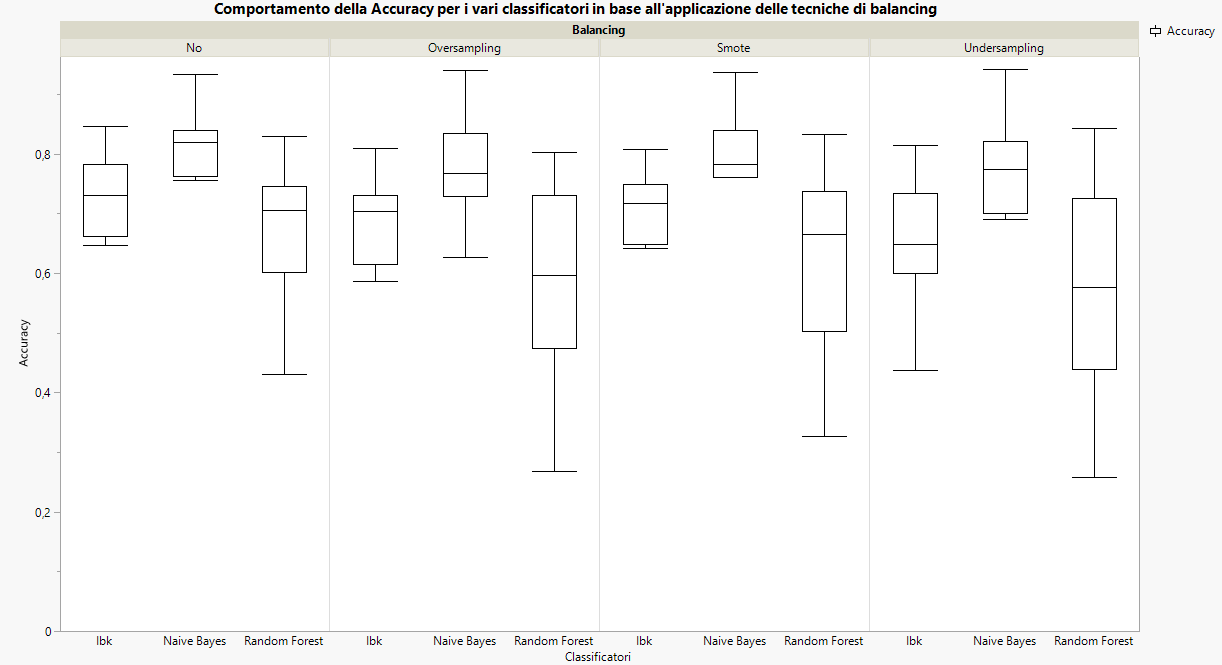
\includegraphics[width=\textwidth]{figs/bookkeeper-accuracy}}
\end{figure}
\end{block}
\end{frame}

\begin{frame}
\frametitle{Bookkeeper - Caso specifico (2/4)}
\begin{block}{Considerazioni sulla accuracy dei classificatori}
\begin{itemize}
\item Si può notare che nel momento in cui viene applicata una qualsiasi tecnica di balancing l'accuratezza di ogni classificatore peggiora
\item Questo risultato non è una sorpresa perché nel testing set si hanno più negativi che positivi (perché nel testing set non si applica il balancing) e il classificatore restituisce più positivi nel caso in cui si applica il balancing 
\item Questo porta a dire che il classificatore sbaglierà tanto
\begin{itemize}
\item aumentano i falsi positivi
\item diminuiscono i falsi negativi
\end{itemize}
\end{itemize}
\end{block}
\end{frame}

\begin{frame}
\frametitle{Zookeeper - Caso specifico (3/4)}
\begin{block}{Recall dei classificatori in base alle tecniche di cost sensitive}
\begin{figure}[ht!]
\frame{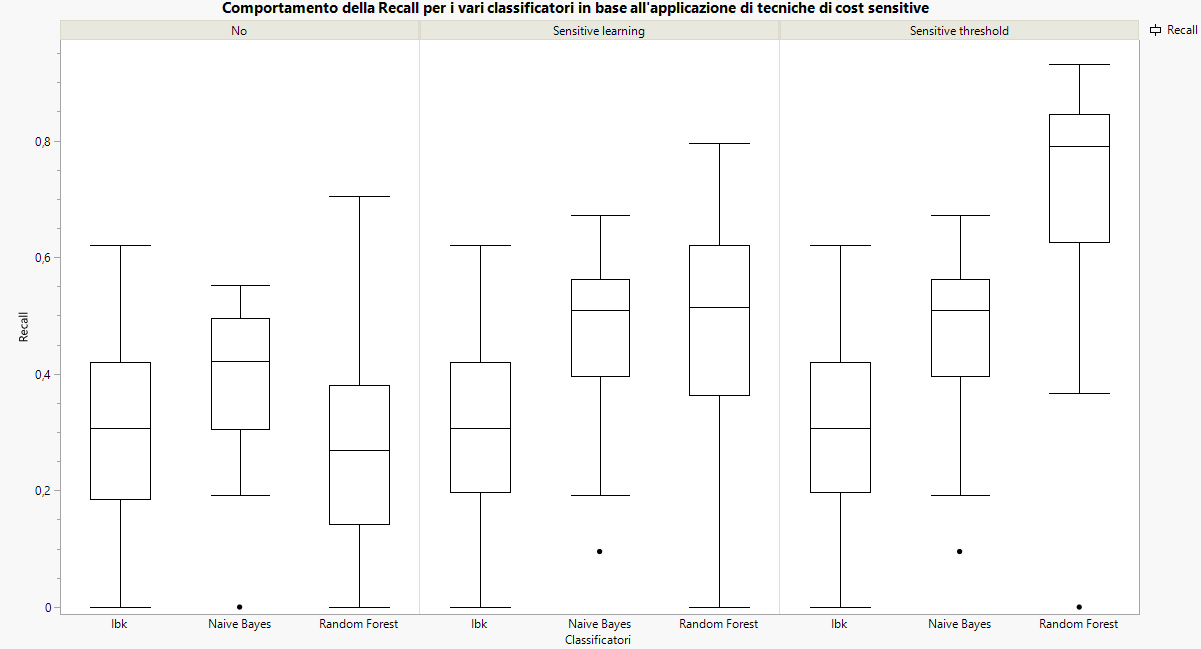
\includegraphics[width=\textwidth]{figs/zookeeper-sensitive}}
\end{figure}
\end{block}
\end{frame}

\begin{frame}
\frametitle{Zookeeper - Caso specifico (4/4)}
\begin{block}{Considerazioni sulla recall dei classificatori}
\begin{itemize}
\item Ad eccezione del classificatore Ibk in cui la \textit{recall} rimane costante, la \textit{recall} migliora nel caso in cui si applicano tecniche di cost sensitive
\item Questo risultato non è una sopresa perché il costo per un falso negativo è dieci volte maggiore di quelle per un falso positivo e quindi l'idea di base è che il classificatore tende a classificare una classe come buggy con più facilità
\end{itemize}
\end{block}
\end{frame}

\section{Conclusioni}
\begin{frame}
\frametitle{Conclusioni}
\begin{itemize}
\item La risposta, in seguito all'analisi dei risultati, è che non esiste il classificatore migliore, ma esso dipende dal contesto in cui ci si trova
\item Nell'ingegneria c'è sempre un compromesso ed infatti bisogna trovare il classificatore adatto alle esigenze che si hanno
\begin{itemize}
\item[--] Ad esempio, si potrebbe volere un valore abbastanza alto di \textit{recall} perché questo porterebbe ad avere un minor rischio di non testare una classe buggy
\end{itemize}
\item Per entrambi i progetti, il classificatore \textit{Random Forest} presenta la \textit{recall} migliore
\item \textit{Naive Bayes} è il classificatore che presenta una \textit{precision} più alta e \textit{AUC} migliore
\end{itemize}
\end{frame}

\section{Repository di lavoro}
\begin{frame}
\frametitle{Repository di lavoro}
\begin{block}{Repository \textit{GitHub}}
La repository \textit{GitHub} contenente il codice sorgente che ha sviluppato i risultati ottenuti è disponibile al seguente link:
\begin{center}
\scriptsize{\url{https://github.com/alessandrochillotti/isw2-deliverable-2.git}}
\end{center}
\end{block}

\begin{block}{Progetto su \textit{SonarCloud}}

L'analisi di \textit{SonarCloud} che mostra come il codice sorgente abbia code smell pari a 0 è disponibile al seguente link:
\begin{center}
\scriptsize{\url{https://sonarcloud.io/project/overview?id=alessandrochillotti_isw2-deliverable-2}}
\end{center}
\end{block}
\end{frame}



\end{document} 
